\documentclass[12pt, letterpaper]{article}
\usepackage{graphicx}
\graphicspath{{GEEJj_kXYAImdwn/}}
\title{My first LaTeX document}
\author{Tom Cat\thanks{Funded by myself}}
\date{March 2024}
\begin{document}
\maketitle
Hello world!
First document. This is a simple example, with no
extra parameters or packages included.
Some of the \textbf{greatest}
discoveries in \underline{science}
were made by \textbf{\textit{accident}}.
Some of the greatest \emph{discoveries} in science 
were made by accident.
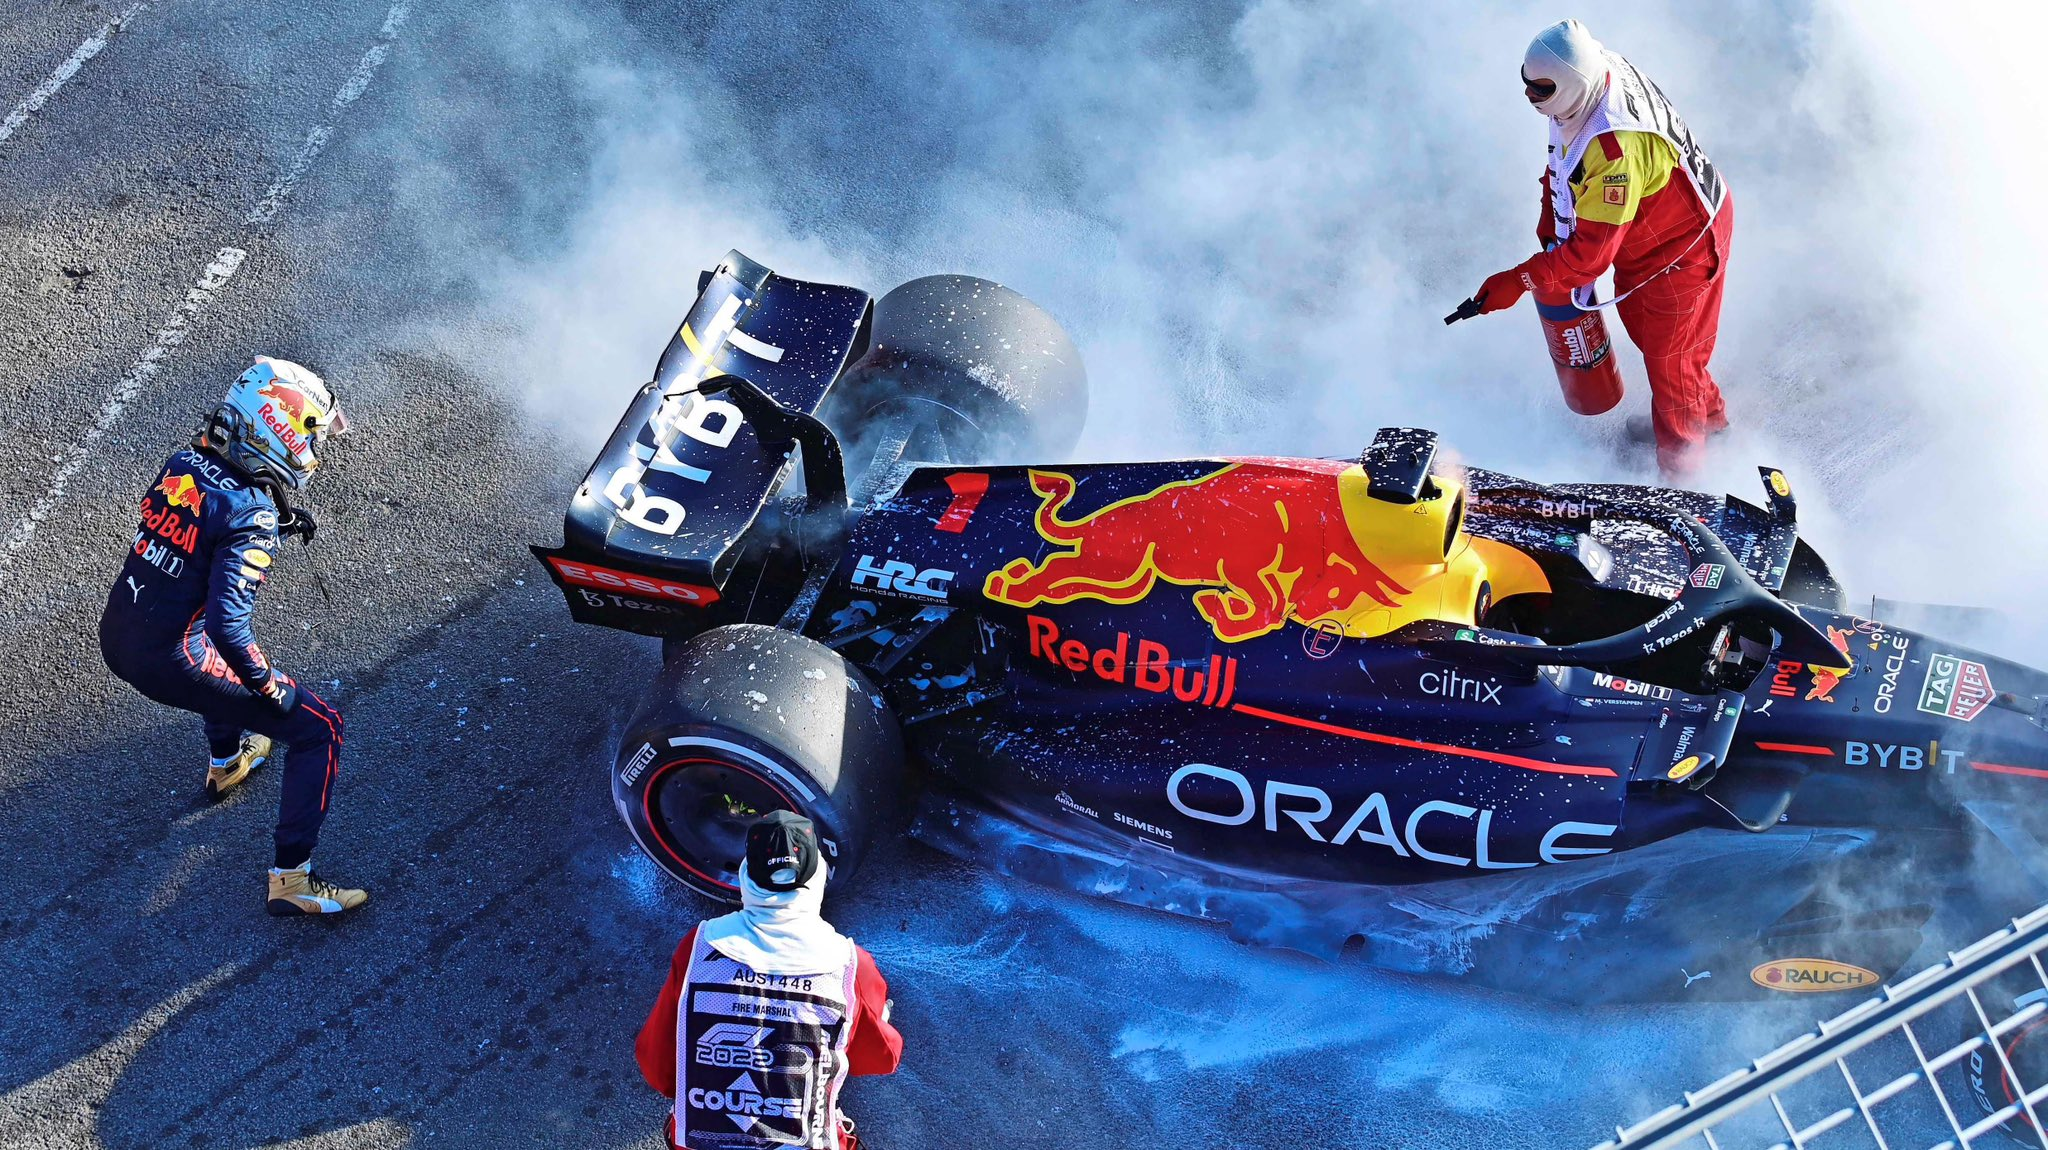
\includegraphics[width=0.5\textwidth]{GEEJj_kXYAImdwn}

\textit{Some of the greatest \emph{discoveries} 
in science were made by accident.}

\textbf{Some of the greatest \emph{discoveries} 
in science were made by accident.}
\end{document}